\section{Value Proposition}
To confirm that the problem and solution definitions match, a value proposition canvass was established.
The hypothethis is made that the customers and the users of this product are different. Indeed the people buying the device will be the family of the elder(s). While the elders will be the end users. Therefore the needs of the buyers and of the users are different. They will be both using the device but through two different interfaces.

The value proposion canvas template used for the analysis is the one pictured in figure \ref{fig:vpcanvas}.

\begin{figure}[!htb]
    \centering
    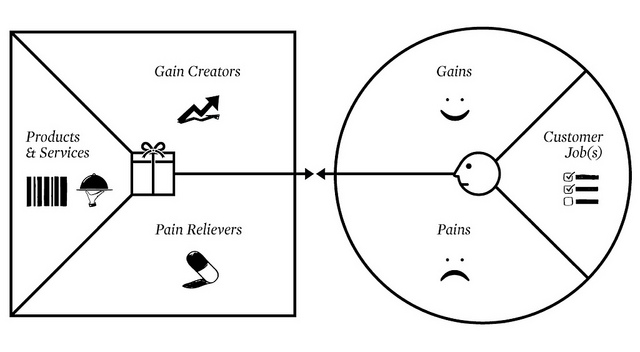
\includegraphics[width=0.6\textwidth,keepaspectratio]{chap/marketFig/vpcanvas.jpg}
    \caption{Business model canvas}
    \label{fig:vpcanvas}
\end{figure}

The value propostion canvas for the elderly can be seen in figure \ref{fig:elders value proposition}. From this canvas the following pain relievers can be link to corresponding pains
\begin{itemize}
  \item{Be included - be forgotten}
  \item{Notification - feel lonely}
  \item{Have an occupation - get bored}
\end{itemize}

The following gain creators match de elderly gains:
\begin{itemize}
  \item{Feel cool - contribute}
  \item{Reinsuring on others state - be informed}
  \item{Feel included - feel loved}
\end{itemize}

Clearly the value map of the device meets the customer profile of the elderly to achieve a fit.
\clearpage
\begin{figure}[!htb]
    \centering
    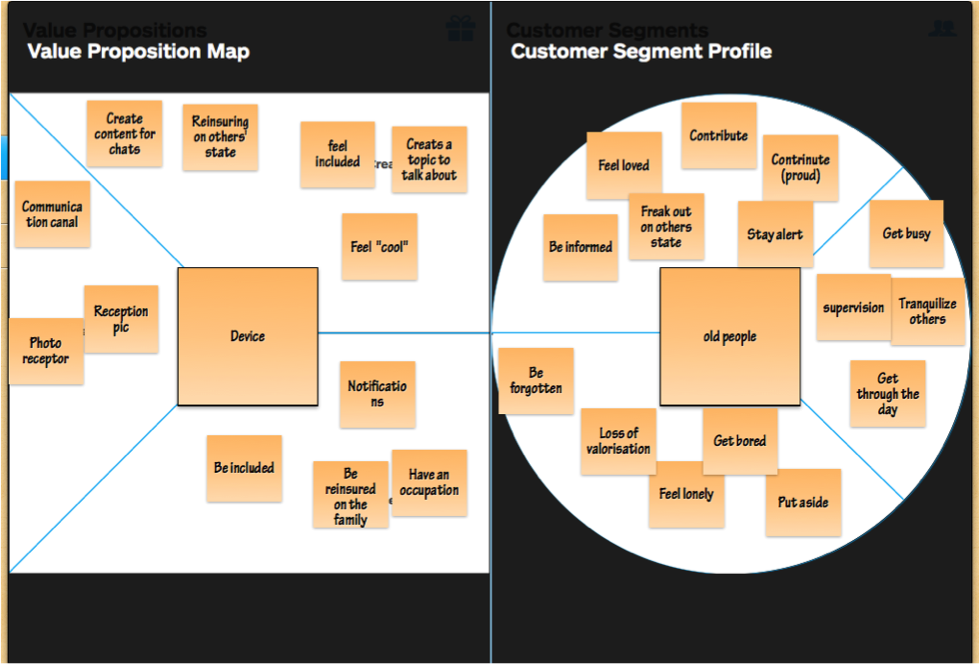
\includegraphics[width=0.9\textwidth,keepaspectratio]{chap/marketFig/elderly_value_prop_canvas.png}
    \caption{Elderly value proposition.}
    \label{fig:elders value proposition}
\end{figure}

The family's main needs are to keep contact easily with their elders even when they cannot be present. To integrate them in their communication habits. To feel less guilty to let them alone. All these things can be achieved with this device.
